% XeLaTeX

\documentclass{article}
\usepackage{ctex}
\usepackage{xypic}
\usepackage{amsfonts,amssymb}
\usepackage{multirow}
\usepackage{geometry}
\usepackage{graphicx}
\usepackage{listings}
\usepackage{lipsum}
\usepackage{courier}
\usepackage{fancyvrb}
\usepackage{etoolbox}


\linespread{1.2}
\geometry{left=3cm,right=2.5cm,top=2.5cm,bottom=2.5cm}

\makeatletter
\patchcmd{\FV@SetupFont}
  {\FV@BaseLineStretch}
  {\fontencoding{T1}\FV@BaseLineStretch}
  {}{}
\makeatother

\lstset{basicstyle=\small\fontencoding{T1}\ttfamily,breaklines=true}
\lstset{numbers=left,frame=shadowbox,tabsize=4}
%\lstset{extendedchars=false}
\begin{document}

\title{实验一 \ 接管裸机的控制权 \ 实验报告}
\author {数据科学与计算机学院 \ 计算机科学与技术 2016 级 \\ 王凯祺 \ 16337233}
\maketitle

\section{实验目的}

\begin{itemize}
\item 掌握 NASM 的语法
\item 掌握用汇编器的用法
\item 掌握创建空白软盘镜像的方法
\item 掌握 WinHex 软件的使用方法
\item 掌握虚拟机的设置及使用方法
\end{itemize}

\section{实验要求}

设计 IBM PC 的一个引导扇区程序,程序功能是:用字符 'A' 从屏幕左边某行位置 45 度角下斜射出,保持一个可观察的适当速度的直线运动,碰到屏幕的边后产生反射,改变方向运动,如此类推,不断运动;在此基础上,增加你的个性扩展。还要在屏幕某个区域以特别的方式显示你的学号姓名等个人信息。将这个程序的机器码放进虚拟软盘的首扇区,并用此软盘引导你的 PC ,直到成功。

\section{实验方案}

本实验需要使用 NASM 汇编器、WinHex 软件和虚拟机。

\subsection{NASM 汇编器的使用}

在 Windows 下打开命令提示符,执行以下命令:

\begin{lstlisting}[language=bash]
name -f bin stone.asm -o stone.com
\end{lstlisting}

如果编译成功,屏幕会显示 Warning 信息或不显示任何内容。

如果编译不成功,屏幕会显示 Error 信息以及 Warning 信息。

\subsection{创建空白软盘镜像}

关于创建空白镜像,我查了一下网上对 flp 格式的解释,只需要在二进制模式下写 $1440 \times 1024$ 字节的 $0$ 即可创建空白镜像。使用 C++ 代码可创建该空白镜像。执行该代码会将新的空白镜像保存在当前目录的 new.flp 文件。

\begin{lstlisting}[language=C++]
#include <bits/stdc++.h>

#define N (1440 * 1024)

using namespace std;

char a[N * 2];

int main() {
	freopen("new.flp", "w", stdout);
	memset(a, 0, sizeof(a));
	fwrite(a, 1, N, stdout);
}

\end{lstlisting}

\subsection{使用 WinHex 软件修改镜像}

\begin{itemize}
\item 用 WinHex 打开编译好的 COM 文件、空白的 flp 镜像
\item 将 COM 文件全文复制到 flp 镜像的 0x0000 字节处,须保证文件大小不变
\item 将 0x01FE, 0x1FF 两个字节的值分别修改为 0x55, 0xAA
\end{itemize}

\subsection{虚拟机的配置}

实验环境:

\begin{itemize}
\item 操作系统环境 Ubuntu 16.10
\item 虚拟机环境 VirtualBox 5.2.4 r1 19785 (Qt5.6.1)
\end{itemize}

虚拟机配置:

\begin{itemize}
\item 操作系统: 其他 - DOS
\item CPU: 1 核心
\item 内存: 32 MB
\item 显存: 9 MB
\item 软盘: 使用镜像文件 a.flp
\end{itemize}

\section{实验过程和结果}

\subsection{汇编程序的修改}

\subsubsection{删除程序段}

我们直接编译老师提供的代码,发现编译错误如下:

\begin{figure}[!hbp]
	\centering
	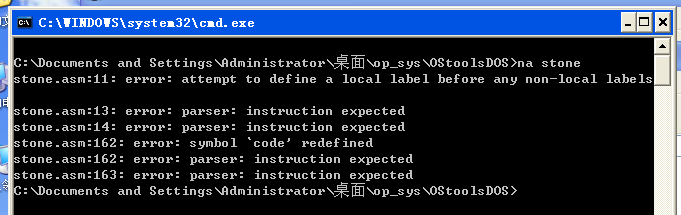
\includegraphics[scale=0.6]{pics/1.png}
\end{figure}

\begin{lstlisting}[language={[x86masm]Assembler}]
     .386
     org 100h					; 程序加载到100h,可用于生成COM
     ASSUME cs:code,ds:code
code SEGMENT
\end{lstlisting}

以上程序的 1 - 4 行为原程序的 11 - 14 行。

我看到这几条编译错误是一脸懵的,并不知道出了什么问题。

于是我把编译的错误信息敲到 Google 里搜索,找到了一个以前的问题:

https://stackoverflow.com/questions/11572307/nasm-error-parsing-instruction-expected?lq=1

\begin{figure}[!hbp]
	\centering
	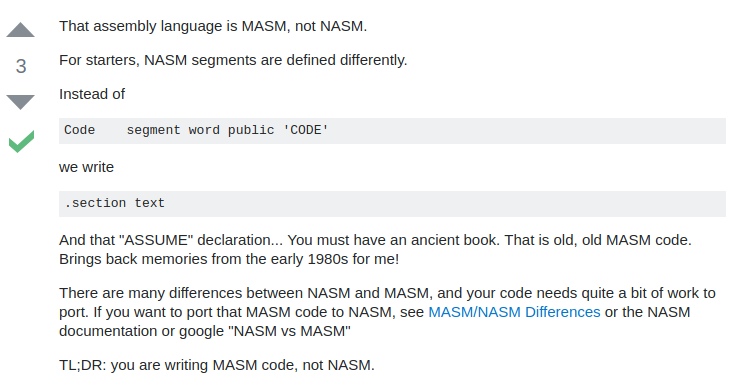
\includegraphics[scale=0.6]{pics/2.png}
\end{figure}

上面的解答非常精彩,大意是说:这是 MASM 代码,不可以用 NASM 编译。如果要使用 NASM 编译,须将代码段删除,或者换成 NASM 规定的代码段(section .text)。答主还调侃了 MASM 是上世纪 80 年代的东西,题主提的问题仿佛让我看到了一本古书。回答的最后还附有 MASM 和 NASM 的差别。

所以最后,我对这个问题的处理方式是:

\begin{itemize}
\item 删除 11 行、 13 行、 14 行、 162 行、 163 行
\item 在原程序的 15 行前加上 section .text
\item 在原程序的 155 行前加上 section .data
\end{itemize}

\subsubsection{修改显示地址}

修改了上述问题后,程序终于能编译通过了。我迫不及待点开来看,发现啥也没显示。

于是我立刻怀疑 show 模块有鬼。

果然不出所料, es 为 0 ,与显示的起始地址 0xB8000 不匹配。

由于之前已设置了初值 gs = 0xB800 ,我把 es 换成 gs 就解决了此问题。

\begin{figure}[!hbp]
	\centering
	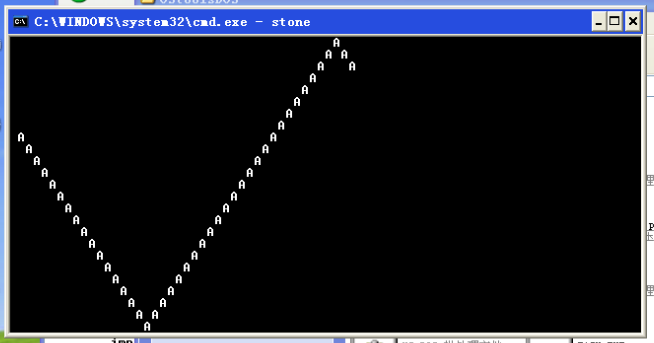
\includegraphics[scale=0.6]{pics/3.png}
\end{figure}

修改以上代码,老师写的程序就成功地运行在我的 Windows XP 上了!

\subsubsection{加入个性化信息}

我想把单个字符 'A' 换成自己的名字、学号,就在数据段写了一个字符串。每次刷新屏幕时,用字符串指针 si 寄存器从头到尾遍历字符串,在屏幕上显示的就是我的学号和姓名信息了!

\subsubsection{减小程序体积}

程序写好后,我发现我的可执行文件大小为 519 字节,大于规定的 510 字节,导致 511 - 512 字节处无法填写 0x55AA 。经过对代码的细致检查,我发现有几条没用的语句,将其删除后把可执行文件的大小控制在 507 字节。

\subsection{写入 flp 软盘镜像}

\begin{itemize}
\item 用 WinHex 打开编译好的 COM 文件、空白的 flp 镜像
\item 将 COM 文件全文复制到 flp 镜像的 0x0000 字节处,须保证文件大小不变
\item 将 0x01FE, 0x1FF 两个字节的值分别修改为 0x55, 0xAA
\end{itemize}

\subsection{用虚拟机执行程序}

将 flp 软盘镜像挂载到虚拟机上,即可运行程序。

\subsubsection{修复初始化问题}

老师写的程序能运行在 Windows XP 上,但是在虚拟机却不能正确运行,如下图,只有一个光标在显示。

\begin{figure}[!hbp]
	\centering
	
\includegraphics[scale=0.6]{pics/4.png}
\end{figure}

我感到非常奇怪,决定去探个究竟。

我决定写一个简单的程序在虚拟机上跑:

\begin{lstlisting}[language={[x86masm]Assembler}]
    org 100h					; 程序加载到100h,可用于生成COM
start:
    mov ax,cs
	mov es,ax					; ES = 0
	mov ds,ax					; DS = CS
	mov es,ax					; ES = CS
	mov ax,0B800h				; 文本窗口显存起始地址
	mov gs,ax					; GS = B800h
    mov byte[char],'A'
show:	
    xor ax,ax                 ; 计算显存地址
    mov ax,word[x]
	mov bx,80
	mul bx
	add ax,word[y]
	mov bx,2
	mul bx
	mov bx,ax
	mov ah,0Fh				;  0000:黑底、1111:亮白字(默认值为07h)
	mov al,byte[char]			;  AL = 显示字符值(默认值为20h=空格符)
	mov [gs:bx],ax  		;  显示字符的ASCII码值
end:
    jmp $                   ; 停止画框,无限循环 
	
datadef:
    x    dw 7
    y    dw 0
    char db 'A'
\end{lstlisting}

这一跑,就跑出问题来了!屏幕上显示了 'A' 字符,只是它是在左上角 (0, 0) 位置,与我们预期的 (7, 0) 位置不符。我怀疑是汇编程序没有帮我初始化,就在第 10 行前加上两行:

\begin{lstlisting}[language={[x86masm]Assembler}]
	mov word [x], 7
	mov word [y], 0
\end{lstlisting}

修改后,成功在虚拟机上运行! NASM 程序在虚拟机运行时确实没有初始化变量。

\subsubsection{后续}

舍友告诉我,裸机上程序入口应为 0x7c00 ,而不是 0x0100 ,所以变量没有初始化。

于是我把 org 100h 改为 org 7c00h ,并把变量初始化的过程删掉,顺利在虚拟机上运行。

\newpage

\subsection{最终运行效果图}

\subsubsection{某一帧的画面}

\begin{figure}[!hbp]
	\centering
	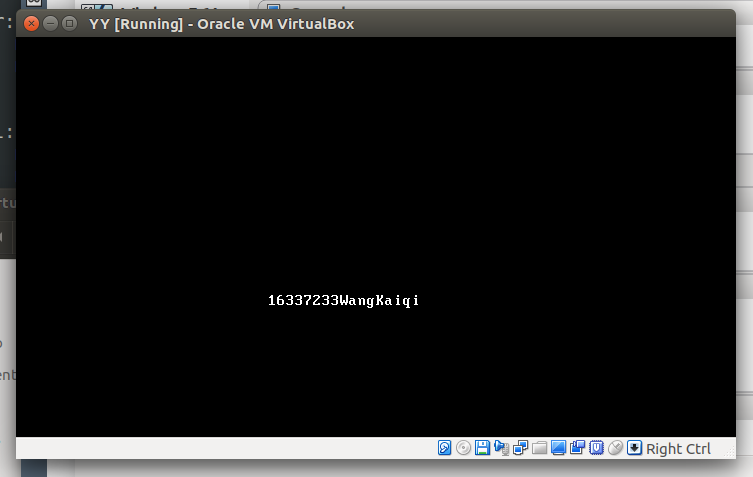
\includegraphics[scale=0.5]{pics/5.png}
\end{figure}

\subsubsection{运行轨迹图}

\begin{figure}[!hbp]
	\centering
	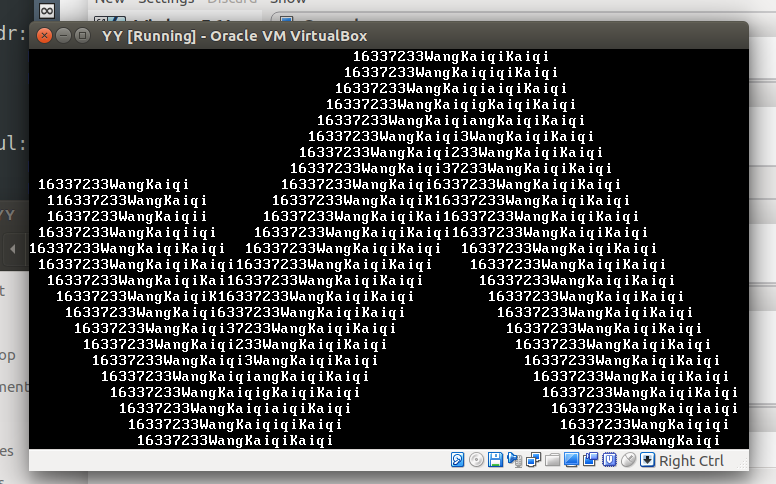
\includegraphics[scale=0.5]{pics/6.png}
\end{figure}

\section{实验总结}

这次实验的意义很大,因为它锻炼了我的独立动手能力、资料查找能力,也让我了解到了操作系统是如何运行的,了解到 NASM 与 MASM 的区别。

在实验过程中,我遇到了很多的错误,包括无法编译、屏幕上无输出、在虚拟机上无法正确运行。我通过查找资料、自己动手尝试,测试究竟是哪里出问题,找到问题的根源。找到问题的根源还不够,怎么改还是一个挑战。由于汇编语言是上个学期计算机组成原理的内容,里面的指令我都忘得差不多了,同样是需要上网搜索指令的用法。

在我自己遇到问题时,会跟其他同学讨论。我在自己的机器上运行成功,却在舍友的机器上不能正确运行,只能显示光标。舍友告诉我:“你的 0x55AA 与你的可执行程序重叠了。” 我在编写时想着最后那几个字符应该无关紧要,重叠了就让它重叠嘛;后来修改后在舍友的机器上可以运行,更正了我的观点。因为每个字符都是指令的一部分,如果被修改了,指令也会被修改。

在其他同学遇到问题时,我也会指出对方的问题。比如我舍友的软盘镜像只能在他自己的机器上跑,却不能在我的机器上跑,显示 No bootable device 错误。我怀疑是镜像有问题,查看镜像大小,少了 3 个字节。他改好后,再在我的机器上运行,就运行成功了。

总之,这次实验的意义很大,让我不再停留在课本,而是亲身实践,写出一个非常简单的操作系统出来。

\end{document}
















